
%(BEGIN_QUESTION)
% Copyright 2015, Tony R. Kuphaldt, released under the Creative Commons Attribution License (v 1.0)
% This means you may do almost anything with this work of mine, so long as you give me proper credit

Suppose we have a Koyo ``CLICK'' PLC connected to three process switches as shown in this illustration:

$$\includegraphics[width=15.5cm]{i04667x01.eps}$$

Determine the switch stimuli (i.e. required pressure, temperature, and level) given the ``live'' display of the ladder logic program shown here:

$$\includegraphics[width=15.5cm]{i04667x02.eps}$$

Also, determine the status of the lamp connected to the PLC's {\tt Y1} output.

\vskip 20pt \vbox{\hrule \hbox{\strut \vrule{} {\bf Suggestions for Socratic discussion} \vrule} \hrule}

\begin{itemize}
\item{} Identify how you could override the PLC program to force the lamp to energize, if your only tool at hand was a screwdriver.
\end{itemize}

\underbar{file i04667}
%(END_QUESTION)





%(BEGIN_ANSWER)

\noindent
{\bf Partial answer:}

\medskip
%\item{} Pressure switch = {\bf less than 30 PSI}
\item{} Temperature switch = {\bf cooler than 150 deg F}
%\item{} Level switch = {\bf greater than 4 inches}
\medskip

%The lamp will be de-energized.

%(END_ANSWER)





%(BEGIN_NOTES)

\begin{itemize}
\item{} Pressure switch = {\bf less than 30 PSI}
\item{} Temperature switch = {\bf cooler than 150 deg F}
\item{} Level switch = {\bf greater than 4 inches}
\end{itemize}

The lamp will be de-energized.


%INDEX% PLC, relating I/O status to virtual elements 

%(END_NOTES)


